\documentclass{lab}

\newcommand{\Cd}{^{\circ}\mathrm{C}}

\begin{document}

\begin{titlepage}

\pagestyle{empty}	% Нумерация выкл.

\begin{center}
	\textsc{\LARGE Московский Физико-Технический Институт}\\[1,5cm]
	\textsc{\Large Кафедра общей физики}\\[0,5cm]
	\textsc{\large Лабораторная работа \textnumero 3.4.2}\\[2.5cm]

	\noindent\rule{\textwidth}{1pt}
	\\[0.5cm]
	{ \huge \bfseries Закон Кюри-Вейсса}
	\\[0.1cm]
	\noindent\rule{\textwidth}{1pt}
\end{center}

\vfill

\begin{minipage}[b]{0.3\textwidth}
	Маршрут \RomanNumeralCaps{3}\\\\
	20 октября 2018 г.\\
	27 октября 2018 г.
\end{minipage}
\hfill
\begin{minipage}[b]{0.33\textwidth}
	\textit{Работу выполнил}\\
	Ринат Валиев, 711 гр.\\\\
	\textit{Под руководством}\\
	Г.И. Лапушкина, к.ф.-м.н.
\end{minipage}

\end{titlepage}

\pagestyle{VR}
\setcounter{page}{2}

\section*{Постановка эксперимента}

\begin{quote}
\textbf{{\normalsize Цель работы: }}
изучение температурной зависимости магнитной восприимчивости ферромагнетика выше точки Кюри.
\end{quote}

\begin{quote}
\textbf{{\normalsize Оборудование: }}
катушка самоиндукции с образцом из гадолиния, термостат, частотомер, цифровой вольтметр,
$ LC $-автогенератор, термопара медь-константан.
\end{quote}

\subsection*{Теоретическая часть}
\hspace*{\parindent}
Вещества с отличными от нуля атомными магнитными моментами обладают парамагнитными свойствами.
Внешнее магнитное поле ориентирует магнитные моменты, которые в отсутствие поля располагались
в пространстве хаотичным образом.\\
При повышении температуры $ T $ возрастает дезориентирующее действие теплового движения частиц,
магнитная восприимчивость парамагнетиков убывает: в постоянном магнитном поле -- по закону Кюри:
\begin{equation}\label{key1}
\chi = \dfrac{C}{T}, ~~~~~~~ где ~ C ~ - ~ постоянная ~ Кюри.
\end{equation}
\begin{wrapfigure}[12]{r}{3.5cm}
	\vspace{-0.7cm}
	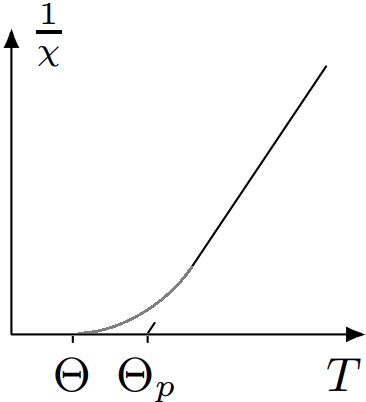
\includegraphics[width=3.5cm]{graph}
	\caption{\footnotesize
	Зависимость обратной величины магнитной восприимчивости от температуры
	}
	\label{graph}
\end{wrapfigure}
\hspace*{\parindent}
Для парамагнитных веществ, которые при понижении температуры становятся ферромагнитными, формула
\eqref{key1} должна быть видоизменена. При $ T \rightarrow 0 $ тепловое движение все меньше
препятствует магнитным моментам атомов ориентироваться в одном направлении при сколь угодно
слабом внешнем поле. В ферромагнетиках это происходит при температуре Кюри $ \Theta $, при этом
применяется закон Кюри-Вейсса:
\begin{equation}\label{key2}
\chi \sim \dfrac{1}{T - \Theta_p}, ~~~~~~~ где ~ \Theta_p ~ - ~ температура, ~ близкая ~ к
~ \Theta.
\end{equation}

Иногда $ \Theta_p $ называют парамагнитной, а $ \Theta $ -- ферромагнитной точками Кюри.

В нашей работе изучается $ \chi(T) $ гадолиния при температурах выше точки Кюри, которая
находится в интервале комнатных температур.

\subsubsection*{Экспериментальная установка}
\hspace*{\parindent}
Схема установки для проверки закона Кюри-Вейсса показана на рис. \ref{setup}.
Исследуемый образец расположен внутри катушки. Температура образца регулируется с помощью
термостата.\\
\hspace*{\parindent}
Обозначим через $ L $ самоиндукцию катушки с образцом и через $ L_0 $ --
самоиндукцию в отсутствие образца. Получим: $ (L - L_0) \sim \chi $. При изменении самоиндукции 
образца меняется период колебаний автогенератора: $ \tau = 2\pi\sqrt{LC} $, $ C $ -- емкость
контура автогенератора.

Период колебаний в отсутствие образца: $ \tau_0 = 2\pi\sqrt{L_0C} $. Тогда имеем соотношение:
$ (L - L_0) \sim (\tau^2 - \tau_0^2) $. Таким образом, $ \chi \sim (\tau^2 - \tau_0^2) $.

Далее следует, что закон Кюри-Вейсса справедлив, если выполнено соотношение:
\begin{equation}
\dfrac{1}{\chi} \sim (T - \Theta_p) \sim \dfrac{1}{\tau^2 - \tau_0^2}.
\end{equation}

Разность температур исследуемого образца и воды в термопаре контролируется с помощью
медно-константановой термопары и цифрового вольтметра. Один из спаев термопары находится
в тепловом контакте с образцом, а другой погружен в воду. Концы термопары подключены к
цифровому вольтметру.

\begin{figure}[H]
	\centering
	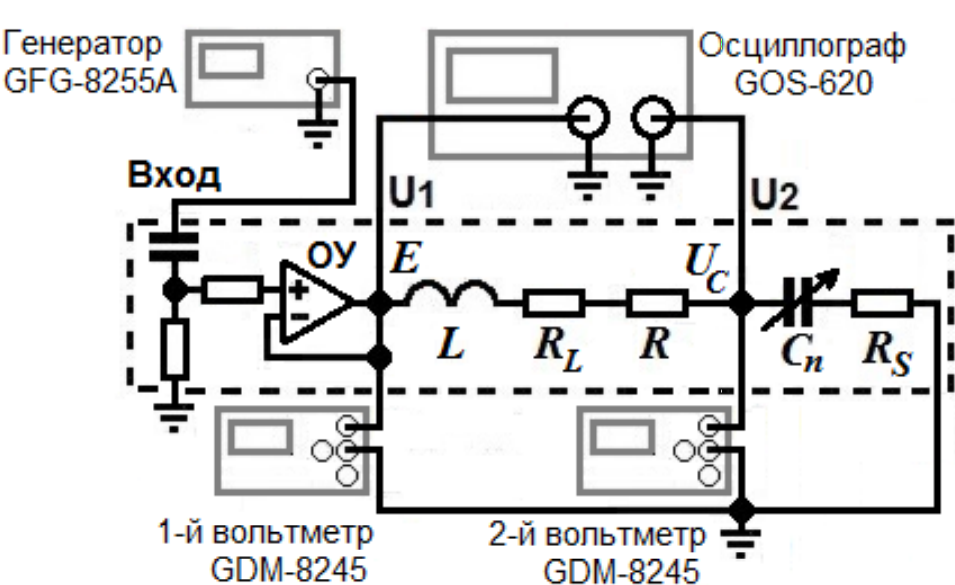
\includegraphics[width = 0.7 \textwidth]{setup}
	\caption{\footnotesize
	Схема экспериментальной установки для проверки закона Кюри-Вейсса\\
	1 - катушка с образцом, 2 - стеклянный сосуд с трансформаторным маслом, 3 - вода в
	термостате, 4 - ртутные термометр, 5 - термостат, 6 - термопара
	}
	\label{setup}
\end{figure}

\section*{Выполнение эксперимента}
\subsection*{Измерения}
\hspace*{\parindent}
В работе исследуется зависимость периода колебаний автогенератора от температуры сердечника
катушки, затем определяется парамагнитная точка Кюри гадолиния.

\begin{enumerate}
\item
Запишем параметры установки: $ k = 24 ~ град/мВ, ~ \tau_0 = 9,045 ~ мкс $.

\item
Исследуем зависимость периода колебаний $ LC $-генератора от температуры образца, отмечая
период колебаний $ \tau $ по частотомеру, а температуру образца $ T $ -- по показаниям дисплея и
цифровому вольтметру ($ \Delta U $ с учетом знака). Термопара подключена так, что при знаке
$ "+" $ на табло вольтметра, температура образца выше температуры рабочей жидкости. Проведем
измерения в диапазоне от~$ 14 \Cd $ до $ 40 \Cd $ через $ 2 \Cd $. Результаты занесем в таблицу
\ref{tab1}.

Для данной таблицы имеем погрешности:
\begin{equation}
\begin{aligned}
&\sigma(T_{изм}) = 0,5~\Cd ~~~~~ \sigma(\Delta U) = 1,2~мкВ ~~~~~ \sigma(\tau) = 0,001~мкс	\\
&\sigma(T) = \sqrt{\sigma(T_{изм})^2 + \sigma(k \cdot \Delta U)^2} = 0,5~\Cd
\end{aligned}
\end{equation}

\newpage

Также в таблицу \ref{tab1} добавим расчеты значений $ (\tau^2 - \tau_0^2) $ и
$ (\tau^2 - \tau_0^2)^{-1} $ с дальнейшей целью построить график $ \chi(T) $ и $ 1/\chi(T) $.

\begin{table}[H]
	\vspace{-0.7cm}
	\centering
	\begin{align}
	&\begin{tabular}{|c|ccccccc|}
		\hline
		N				&1	&2	&3	&4	&5	&6	&7	\\ \hline
		$ T_{изм},~\Cd $&14,03	&16,03	&18,00	&20,02	&22,02	&24,02	&26,02	\\
		$ \Delta U,~мВ $&-17,1	&-18,0	&-7,2	&-17,1	&-16,9	&-16,1	&-16,5	\\
		$ T,~\Cd $		&13,6	&15,6	&17,8	&19,6	&21,6	&23,6	&25,6	\\
		$ \tau,~мкс $	&10,790	&10,701	&10,509	&10,310	&9,980	&9,612	&9,430	\\
		$ (\tau^2 - \tau_0^2) $			&34,612	&32,699	&28,627	&24,484	&17,788	&10,579	&7,113	\\
		$ (\tau^2 - \tau_0^2)^{-1} $	&0,029	&0,031	&0,035	&0,041	&0,056	&0,095	&0,141	\\ \hline
	\end{tabular}\\
	&\begin{tabular}{|c|ccccccc|}
		\hline
		N				&8	&9	&10	&11	&12	&13	&14	\\ \hline
		$ T_{изм},~\Cd $&28,01	&30,01	&32,01	&34,02	&36,01	&38,02	&40,01	\\
		$ \Delta U,~мВ $&-17,0	&-16,3	&-16,0	&-15,2	&-14,7	&-15,0	&-14,0	\\
		$ T,~\Cd $		&27,6	&29,6	&31,6	&33,7	&35,7	&37,7	&39,7	\\
		$ \tau,~мкс $	&10,790	&10,701	&10,509	&10,310	&9,980	&9,612	&9,430	\\
		$ (\tau^2 - \tau_0^2) $			&5,480	&4,492	&3,787	&3,270	&2,920	&2,626	&2,387	\\
		$ (\tau^2 - \tau_0^2)^{-1} $	&0,182	&0,223	&0,264	&0,306	&0,342	&0,381	&0,419	\\ \hline
	\end{tabular}
	\end{align}
	\vspace{-0.5cm}
	\caption{\footnotesize 
		Результаты измерений для зависимости $ \tau(T) $. Также данные для нахождения
		ферромагнитной и парамагнитной точек Кюри через графики $ \chi(T) $ и $ 1/\chi(T) $.
	}
	\label{tab1}
\end{table}

\item
Как уже было отмечено, температура, при которой магнитная восприимчивость резко снижается, почти
до нуля, носит название температуры Кюри -- $ \Theta $. При температурах выше $ \Theta $ процесс
намагничивания ферромагнетика нарушается из-за интенсивного теплового движения атомов и молекул
и материал перестает быть ферромагнитным и становится парамагнетиком.

\begin{figure}[H]
	\centering
	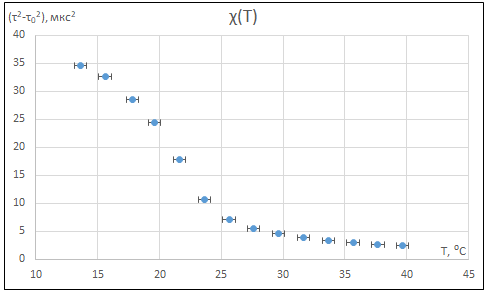
\includegraphics[width = 0.9 \textwidth]{chi}
	\caption{\footnotesize
		График зависимости $ \chi(T) $. Данные из таблицы \ref{tab1}.\\
		$ \left( \chi \sim (\tau^2 - \tau_0^2) \right) $
	}
	\label{chi}
\end{figure}

Из графика $ \chi(T) $ (рис. \ref{chi}) мы не можем определить точку Кюри $ \Theta $ для
гадолиния. Для этого нужно было брать больший диапазон значений температуры, где был бы виден
резкий скачок. Оттуда легко найти~$ \Theta $.

\item
Теперь определим парамагнитную температуру Кюри для гадолиния из зависимости $ 1/\chi(T) $.
\vspace{-0.5cm}
\begin{figure}[H]
	\centering
	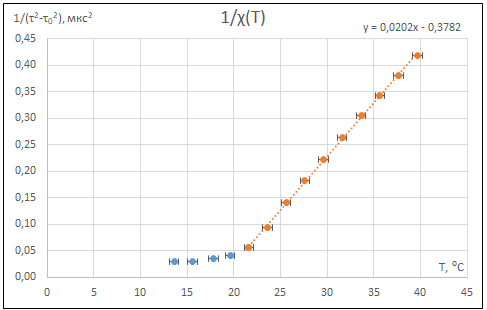
\includegraphics[width = 0.9 \textwidth]{chi-1}
	\caption{\footnotesize
		График зависимости $ 1/\chi(T) $. Данные из таблицы \ref{tab1}.\\
		$ \left( \chi \sim (\tau^2 - \tau_0^2) \right) $
	}
	\label{chi-1}
\end{figure}
\vspace{-0.5cm}
Экстраполируя ту часть графика, где гадолиний ведем себя как парамагнетик, найдем $ \Theta_p $.
Рассмотрев данное линейное уравнение (также записано на рис. \ref{chi-1}) найдем точку
пересечения с осью абсцисс. Результат -- $ 18,7~\Cd $.

Отметим, что для вычисленных значений $ (\tau^2 - \tau_0^2) $ относительная погрешность
меньше $ \varepsilon < 0,1\% $, а также для прямой $ (y = a + bx) $ парамагнитной части кривой
получаются коэффициенты:
\vspace{-0.4cm}
\begin{equation}
\begin{cases}
a = -0,3782		&\varepsilon = 0,3\%	\\
b = 0,0202		&\varepsilon = 0,8\%
\end{cases}
\end{equation}
\end{enumerate}

\section*{Итоги}
\hspace*{\parindent}
В данной работе исследована зависимость магнитной восприимчивости $ \chi $ гадолиния от
температуры выше точки Кюри (табличная $ \Theta = 16~\Cd $). Также рассмотрена зависимость
$ 1/\chi(T) $, откуда определена парамагнитная точка Кюри для гадолиния
$ \Theta_p = (18,7 \pm 1,5)~\Cd $. Относительная погрешность равна $ \varepsilon = 8\% $, что
вполне неплохо. Табличная $ \Theta_p = 20~\Cd $. 

\end{document}